\chapter{Practical Implementation}

\section{Dataset selection}
	T
	
\section{Data preparation}


	\subsection{Data processing and data wrangling}
	
	The data for an invoice and its contained items is stored in an array of objects. This is also shown in code example (\ref{code:JSONSchema}) of a shortened JSON Schema for one invoice. The array "annotations" contains objects. One object represents information such as the invoice date or the unit price. 
	Information about invoice items have labels containing the prefix "lineItem". One invoice containing several items is represented by duplicate values of one label (in the example \ref{code:JSONInvoice} the label "lineItem.description.value"). Here, the order of the labels has to be retained during data wrangling to ensure not mixing up information about different invoice items.

	\lstinputlisting[
	label=code:JSONInvoice,    % Label; genutzt für Referenzen auf dieses Code-Beispiel
	caption=JSON of one invoice,
	captionpos=b,               % Position, an der die Caption angezeigt wird t(op) oder b(ottom)
	style=EigenerPythonStyle,   % Eigener Style der vor dem Dokument festgelegt wurde
	firstline=0,                % Zeilennummer im Dokument welche als erste angezeigt wird
	lastline=23                 % Letzte Zeile welche ins LaTeX Dokument übernommen wird
	]{Quellcode/invoice.json}
	
	The files are processed in python, using the library "json". Each file is opened, and decoded with python's build in json decoder. The hierarchy is traversed until the array "annotations" is reached. Now, the tuples of label and text are saved. This process is split up into invoice and item labels.
	
	The information on invoices is stored in a tabular data structure, a python pandas DataFrame. Worth mentioning is that some invoices contain more information than others. In this case, invoices are still appended into one table, but fields for non-existent values are left empty. The filename is the unique identificator for one invoice.
	
	\begin{figure}[ht]
		\centering
		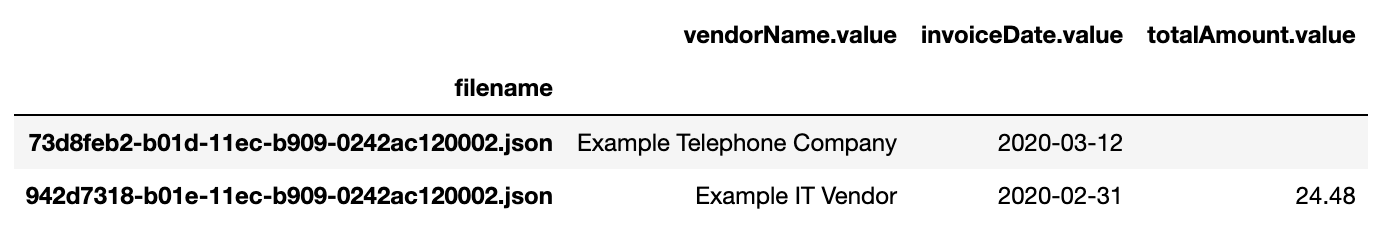
\includegraphics[height=2.5cm]{Bilder/practical/df_invoices.png}
		\caption{Exemplary depiction for processed invoices in a DataFrame}
		\label{fig:df-invoices}
	\end{figure}

	Similarly, information on the invoice items is retrieved from the documents and stored in a pandas DataFrame. Every invoice item has an unique id and can be linked to the respective invoice through the filename.
	
	\begin{figure}[ht]
		\centering
		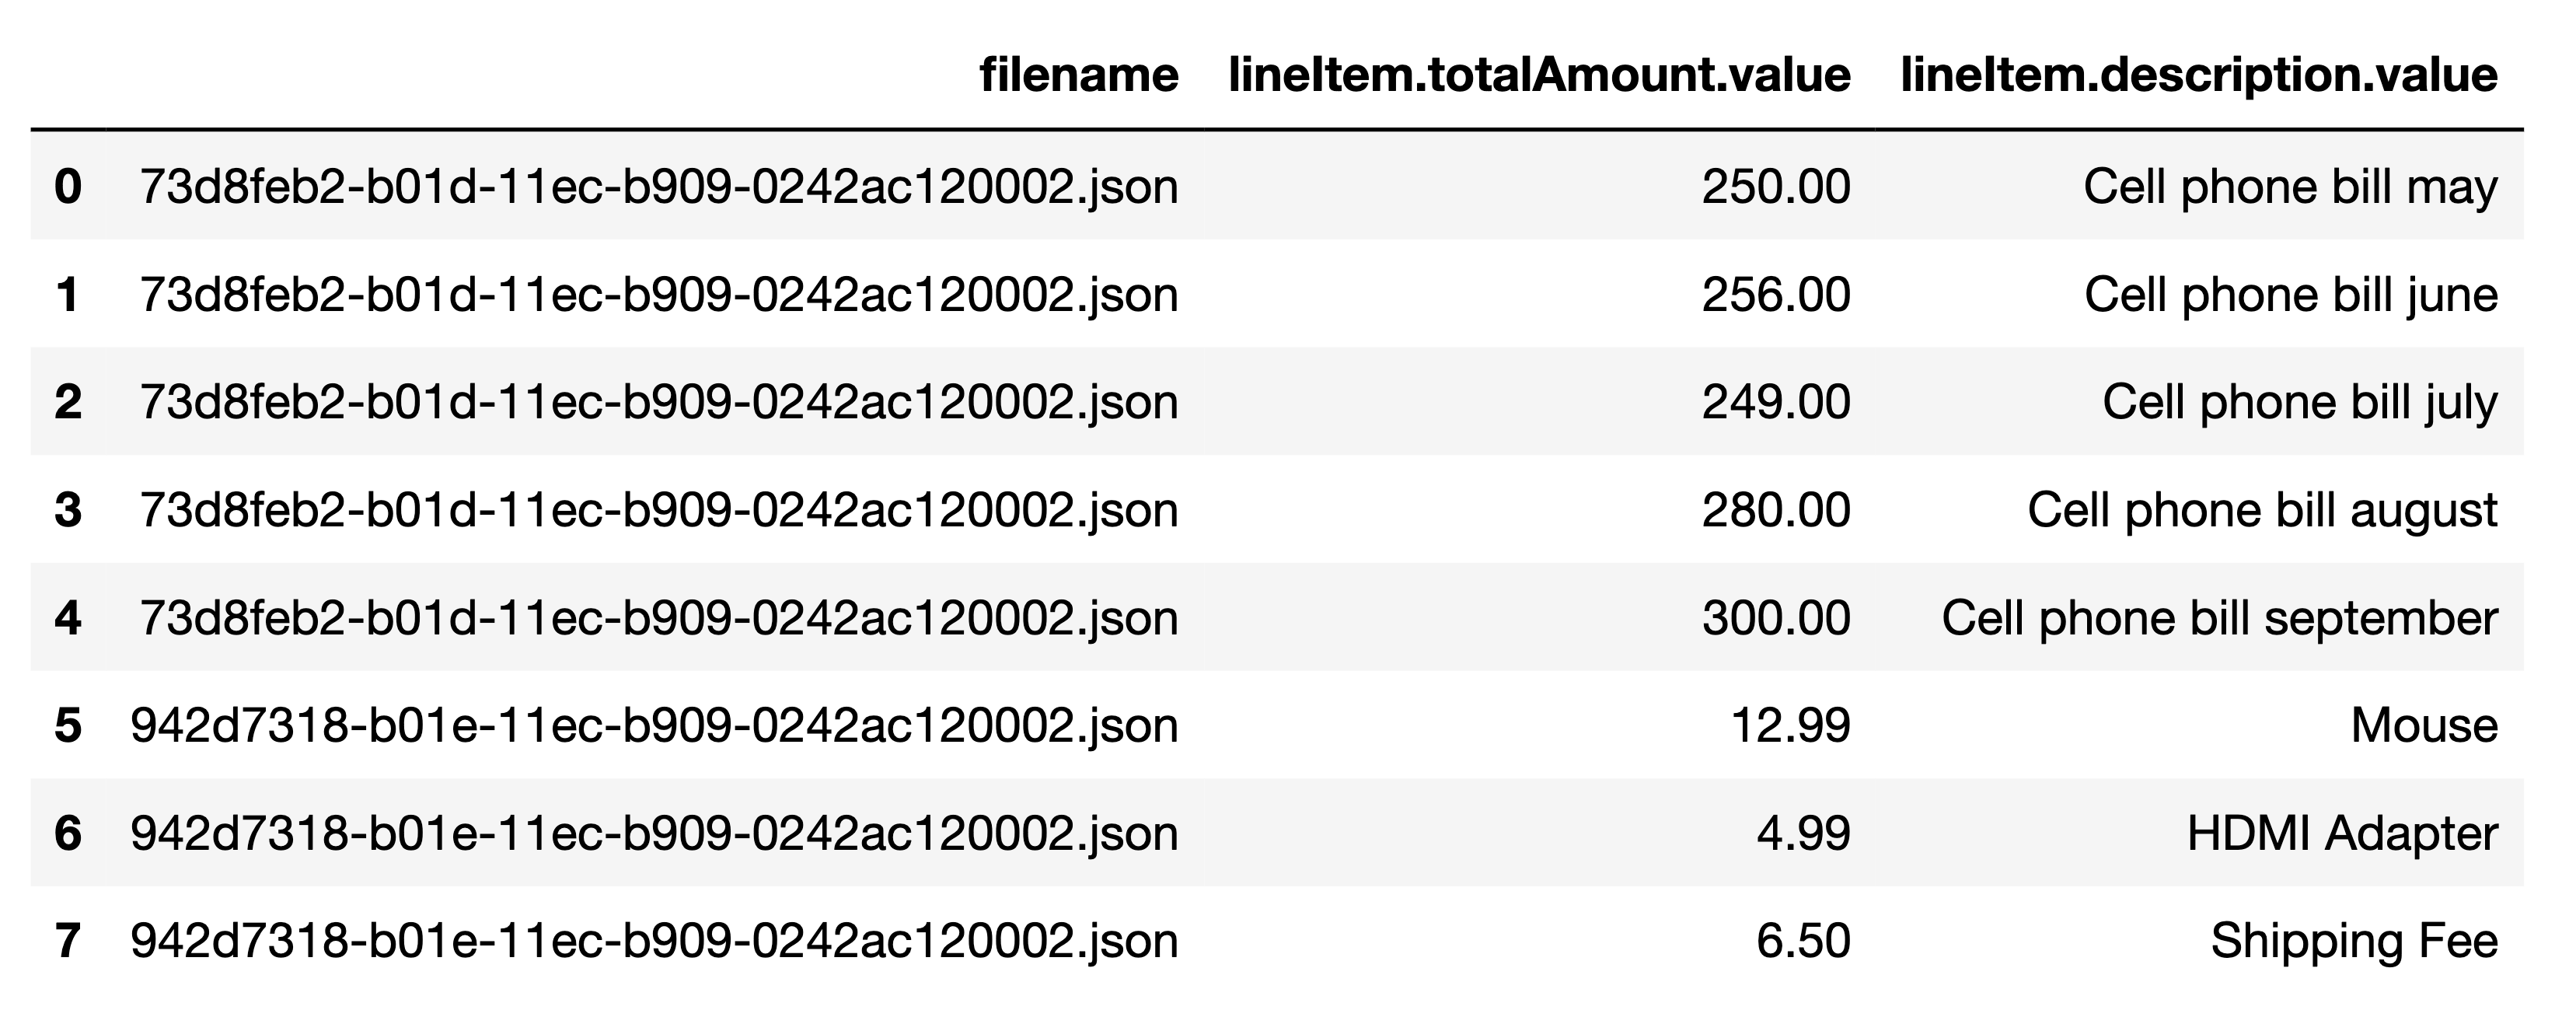
\includegraphics[height=6cm]{Bilder/practical/df_lineitems.png}
		\caption{Exemplary depiction for processed invoice items in a DataFrame}
		\label{fig:df-invoices}
	\end{figure}
	
	The resulting two DataFrames are serialized with the python standard library "pickle".  The data can be efficiently loaded into memory and reserialized again with this library.
	
	This processing step allowed for storing the initial 5.12GB of data in a more usable format and takes up only a total of 393MB. Even further improvements to storage will be dicussed later on.

	The process of reading files from the disk is not inherently an expensive one, but in the realms of many thousand documents, processing times soon reach several days. Observing the execution of the python code showed a peculiarity: While the utilization of the used processor was consequently at the maximum, only one process is executed, leaving the total CPU usage at only 20\%. 
	
	\begin{figure}[ht]
		\centering
		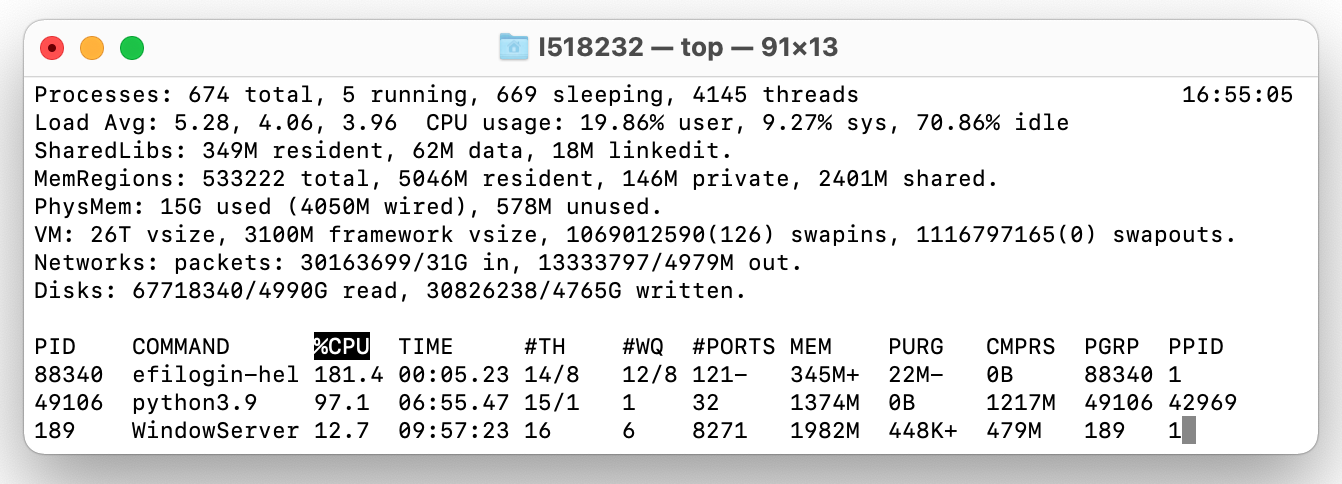
\includegraphics[height=4cm]{Bilder/practical/python_processes.png}
		\caption{Exemplary depiction for processed invoice items in a DataFrame}
		\label{fig:df-invoices}
	\end{figure}
	
	
	One question that may now arise is: Why doesn't python split up the workload and employ the full capacity of the machine?
	This can be explained with the design of the Python interpreter. The \ac{GIL} controls access to the Python Virtual Machine executing the code. This lock only allows exactly one thread to run at a time \cite{corePython}. This of course is not favorable, as valuable CPU capacity is unused. Fortunately, the \ac{GIL} behaves in a special way regarding C code, and I/O operations in Python utilize C code: the lock is released before executing a C routine \cite{corePython}. This allows to bypass the (in this case) inconvenient locking mechanism. 
	
	Different python libraries exploit this speciality and allow to spawn a pool of different processes, which then execute calls asynchronously. One example is the ProcessPoolExecutor. A notable restriction is that only picklable objects can be submitted for multiprocessing. This concerns both fuction and its parameters. While this is not a problem in this task, this restriction will become important later on in the section about feature extraction.
	
	\lstinputlisting[
	label=code:JSONSchema,    % Label; genutzt für Referenzen auf dieses Code-Beispiel
	caption=Shortened JSON Schema of one invoice document representation,
	captionpos=b,               % Position, an der die Caption angezeigt wird t(op) oder b(ottom)
	style=EigenerPythonStyle,   % Eigener Style der vor dem Dokument festgelegt wurde
	firstline=0,                % Zeilennummer im Dokument welche als erste angezeigt wird
	lastline=23                 % Letzte Zeile welche ins LaTeX Dokument übernommen wird
	]{Quellcode/json-schema.json}
	
	

	
	\subsection{Data cleaning}
	
	The task of data cleaning was also completed using python scripts. The library \ac{NLTK}
	
	\begin{lstlisting}[language=sh]
$ python3 -c 'import cleaner; print(cleaner.clean("500grams of special baking flour type 504"))' 
>>>  ['of', 'special', 'baking', 'flour', 'type']
	\end{lstlisting}
	 

	
	
	\subsection{Considerations of Space and Time Complexity}
	The dataset consists of over 150.000 invoices, and in those invoices, over 350.000 items are listed. 
	With hardware-limitation in place, an optimized approach for storing and processing the data is required. 
	Several considerations for speeding up processing time and reducing storage space can be made. 
	In the following, the observations are explained and approaches for improvement are given.

		\subsubsection{Duplicates and space complexity}
		Investigation shows, there are only 79.741 unique descriptions for the listed items. By saving only the unique values, the required space is reduced to less than one fourth compared to before. Additionally, this step is required by most machine learning models, as duplicate input values can skew the outcome. The model is chosen later, so this processing step leaves the model selection more open to different kinds of learning algorithms.
		
		\subsubsection{Reconstructing Relationships and time complexity of searching}
		After the deletion of duplicate descriptions (documents in the corpus), the 
		
		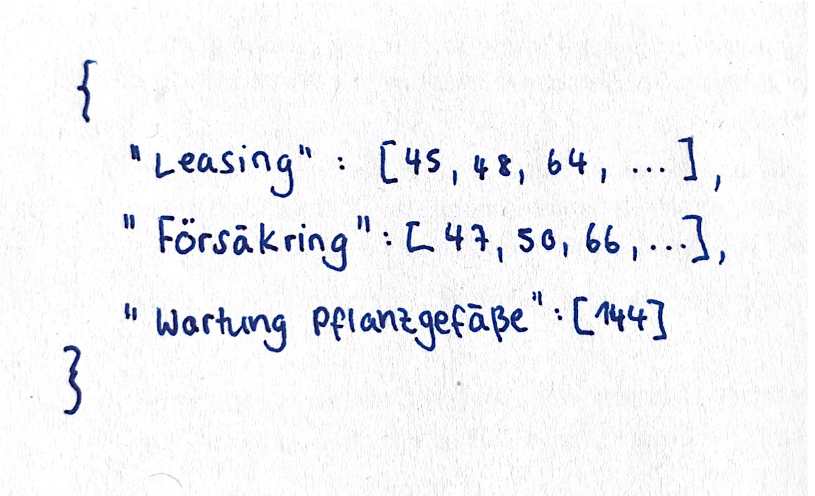
\includegraphics[height=8cm]{Bilder/description_map.png}

	\subsection{Feature Extraction and Feature Engineering}

\section{Modelling}
\section{Evaluation}
	\subsection{Visualization}
\section{Deployment}